\documentclass[conference]{IEEEtran}
\IEEEoverridecommandlockouts
\usepackage[utf8]{inputenc}
\usepackage[T1]{fontenc}
\usepackage[spanish,es-noshorthands,es-tabla]{babel}
\usepackage{cite}
\usepackage{amsmath,amssymb}
\usepackage{graphicx}
\usepackage{booktabs}
\usepackage{url}
\usepackage[hidelinks]{hyperref}
\graphicspath{{../../reports/figures/}{../}{../../reports/experiments/}}

\begin{document}

\title{TRM Predict: sistema de analítica predictiva nativo en la nube para decisiones ante el riesgo cambiario en Colombia}

\author{
\IEEEauthorblockN{Sebastián Cubides, Nicolás Vergara, Edgar Ruiz}
\IEEEauthorblockA{\textit{Ingeniería de Datos e Inteligencia Artificial, V semestre}\\
\textit{Universidad Santo Tomás}, Tunja, Colombia\\
Proyecto integrador: Minería de Datos, Machine Learning y Cloud Computing --- 2026-2}
}

\maketitle

\begin{abstract}
Los hogares que reciben remesas y las micro, pequeñas y medianas empresas (mipymes) importadoras en Colombia están expuestos a la volatilidad de la tasa de cambio peso--dólar (TRM) sin las herramientas analíticas de las grandes empresas. Presentamos \emph{TRM Predict}, un sistema de apoyo a decisiones nativo en la nube que pronostica, para el siguiente día hábil, la dirección de la TRM, su valor esperado y la probabilidad de un movimiento fuerte. Un pipeline CRISP-DM integra la TRM oficial, ocho series de mercado, dos criptoactivos y un índice de sentimiento de noticias obtenido por web scraping en un conjunto de datos sin fuga de información de 2.159 días y 43 variables. La minería no supervisada identifica tres regímenes de mercado, 57 días anómalos y reglas de asociación con lift de hasta 1,24. De 19 modelos optimizados, solo los ensembles superan el azar fuera de muestra: Gradient Boosting alcanza un ROC-AUC de prueba de 0,566 en dirección y 0,586 en riesgo, y un RMSE de regresión 2,4~\% menor que el del paseo aleatorio; una simulación de un hogar con remesas convierte la señal de dirección en una ganancia positiva frente a vender siempre de inmediato. El sistema opera en AWS y está descrito por completo en Terraform (64 recursos): ingesta serverless, data lake en S3 replicado entre regiones, PostgreSQL en RDS y una API en contenedores detrás de un balanceador con auto-scaling en dos zonas de disponibilidad. Los experimentos muestran que, con al menos una instancia por zona, terminar un servidor no produce ninguna petición fallida (100~\% de disponibilidad frente a 77,8~\% con un mínimo de una instancia), y que escalar de dos a cuatro instancias aumenta el rendimiento en 84~\% y reduce la latencia mediana en 60~\%. El proyecto contribuye al ODS~8 (meta 8.10) y al ODS~10 (meta 10.c).
\end{abstract}

\begin{IEEEkeywords}
computación en la nube, minería de datos, aprendizaje automático, CRISP-DM, aprendizaje por ensambles, pronóstico de tasa de cambio, infraestructura como código, desarrollo sostenible
\end{IEEEkeywords}

\section{Introducción}
La \emph{Tasa Representativa del Mercado} (TRM) es la tasa de cambio oficial COP/USD que certifica a diario la Superintendencia Financiera de Colombia. De ella dependen el precio de los bienes importados, el valor de las remesas que reciben los hogares y el costo de la deuda en dólares. Entre septiembre de 2017 y octubre de 2026 se movió entre 2.705 (abril de 2018) y 5.061 COP/USD (noviembre de 2022); solo en 2025 osciló entre 3.707 y 4.417, una variación del 19~\%, y el 18~\% de los días hábiles de la muestra registra una variación superior al 1~\%.

Las grandes empresas cubren este riesgo con mesas de tesorería y derivados, mientras que los hogares y las mipymes suelen decidir por intuición. Las remesas hacia Colombia superaron los USD~11.800 millones en 2024~\cite{banrep_remesas}, de modo que elegir mejor \emph{cuándo} convertir los dólares tiene un efecto tangible en el ingreso familiar. Por ello el proyecto atiende la Agenda 2030~\cite{un2015}: ODS~8 (meta 8.10, acceso a servicios financieros) y ODS~10 (meta 10.c, reducir el costo de las remesas).

\textbf{Contribuciones.} (i) Un pipeline KDD/CRISP-DM reproducible sobre fuentes públicas heterogéneas, con un web scraper diseñado para el problema; (ii) una comparación honesta de 19 modelos de regresión y clasificación frente a las líneas base de paseo aleatorio y clase mayoritaria, con explicaciones SHAP y LIME y una evaluación orientada a decisiones; (iii) un despliegue en AWS de estilo productivo, escrito por completo como Infraestructura como Código, con escalabilidad, disponibilidad y costo medidos.

\section{Planteamiento del problema}
\textbf{Usuarios.} Hogares que reciben remesas, mipymes importadoras y programas de educación financiera. \textbf{Pregunta.} Usando solo datos públicos disponibles antes de que se publique la siguiente TRM, ¿se puede estimar (a) la probabilidad de que suba, (b) su valor esperado y (c) la probabilidad de un movimiento anormalmente fuerte, de forma verificablemente mejor que líneas base ingenuas, y explicar cada predicción? Las tasas de cambio son muy difíciles de pronosticar: Meese y Rogoff mostraron que los modelos estructurales no superan a un paseo aleatorio fuera de muestra~\cite{meese1983}. Por eso, el paseo aleatorio y la clase mayoritaria son líneas base obligatorias en este trabajo.

\section{Trabajos relacionados}
Henrique \emph{et al.}~\cite{henrique2019} revisan el aprendizaje automático para predecir mercados financieros y reportan el predominio de las máquinas de vectores de soporte y las redes neuronales, con los ensembles ganando terreno; Sezer \emph{et al.}~\cite{sezer2020} revisan el aprendizaje profundo para series financieras y destacan su baja interpretabilidad y reproducibilidad. La mayoría de estudios aborda pares de monedas principales o índices bursátiles y se queda en la evaluación fuera de línea. Este trabajo se enfoca en una moneda emergente, usa determinantes propios del país (petróleo, monedas pares, noticias locales), privilegia ensembles interpretables explicados con SHAP~\cite{lundberg2017} y LIME~\cite{ribeiro2016}, y entrega un servicio desplegado y reproducible.

\section{Visión general del sistema}
La Fig.~\ref{fig:arch} muestra el sistema. Cada día hábil a las 18:30 (hora de Colombia), una regla de EventBridge dispara la Lambda de \emph{ingesta}, que consulta la API de datos abiertos de la TRM, Yahoo Finance y Binance, hace scraping de \emph{La República} y escribe un paquete JSON en la zona \emph{raw} de un data lake en S3. Ese objeto dispara la Lambda de \emph{ETL}, que carga los datos en PostgreSQL. Los modelos se entrenan fuera de línea con el pipeline que se describe a continuación y se publican en S3. Un servicio FastAPI en Docker ofrece predicciones, escenarios hipotéticos y un tablero web (Fig.~\ref{fig:dash}).

\begin{figure*}[t]
\centering
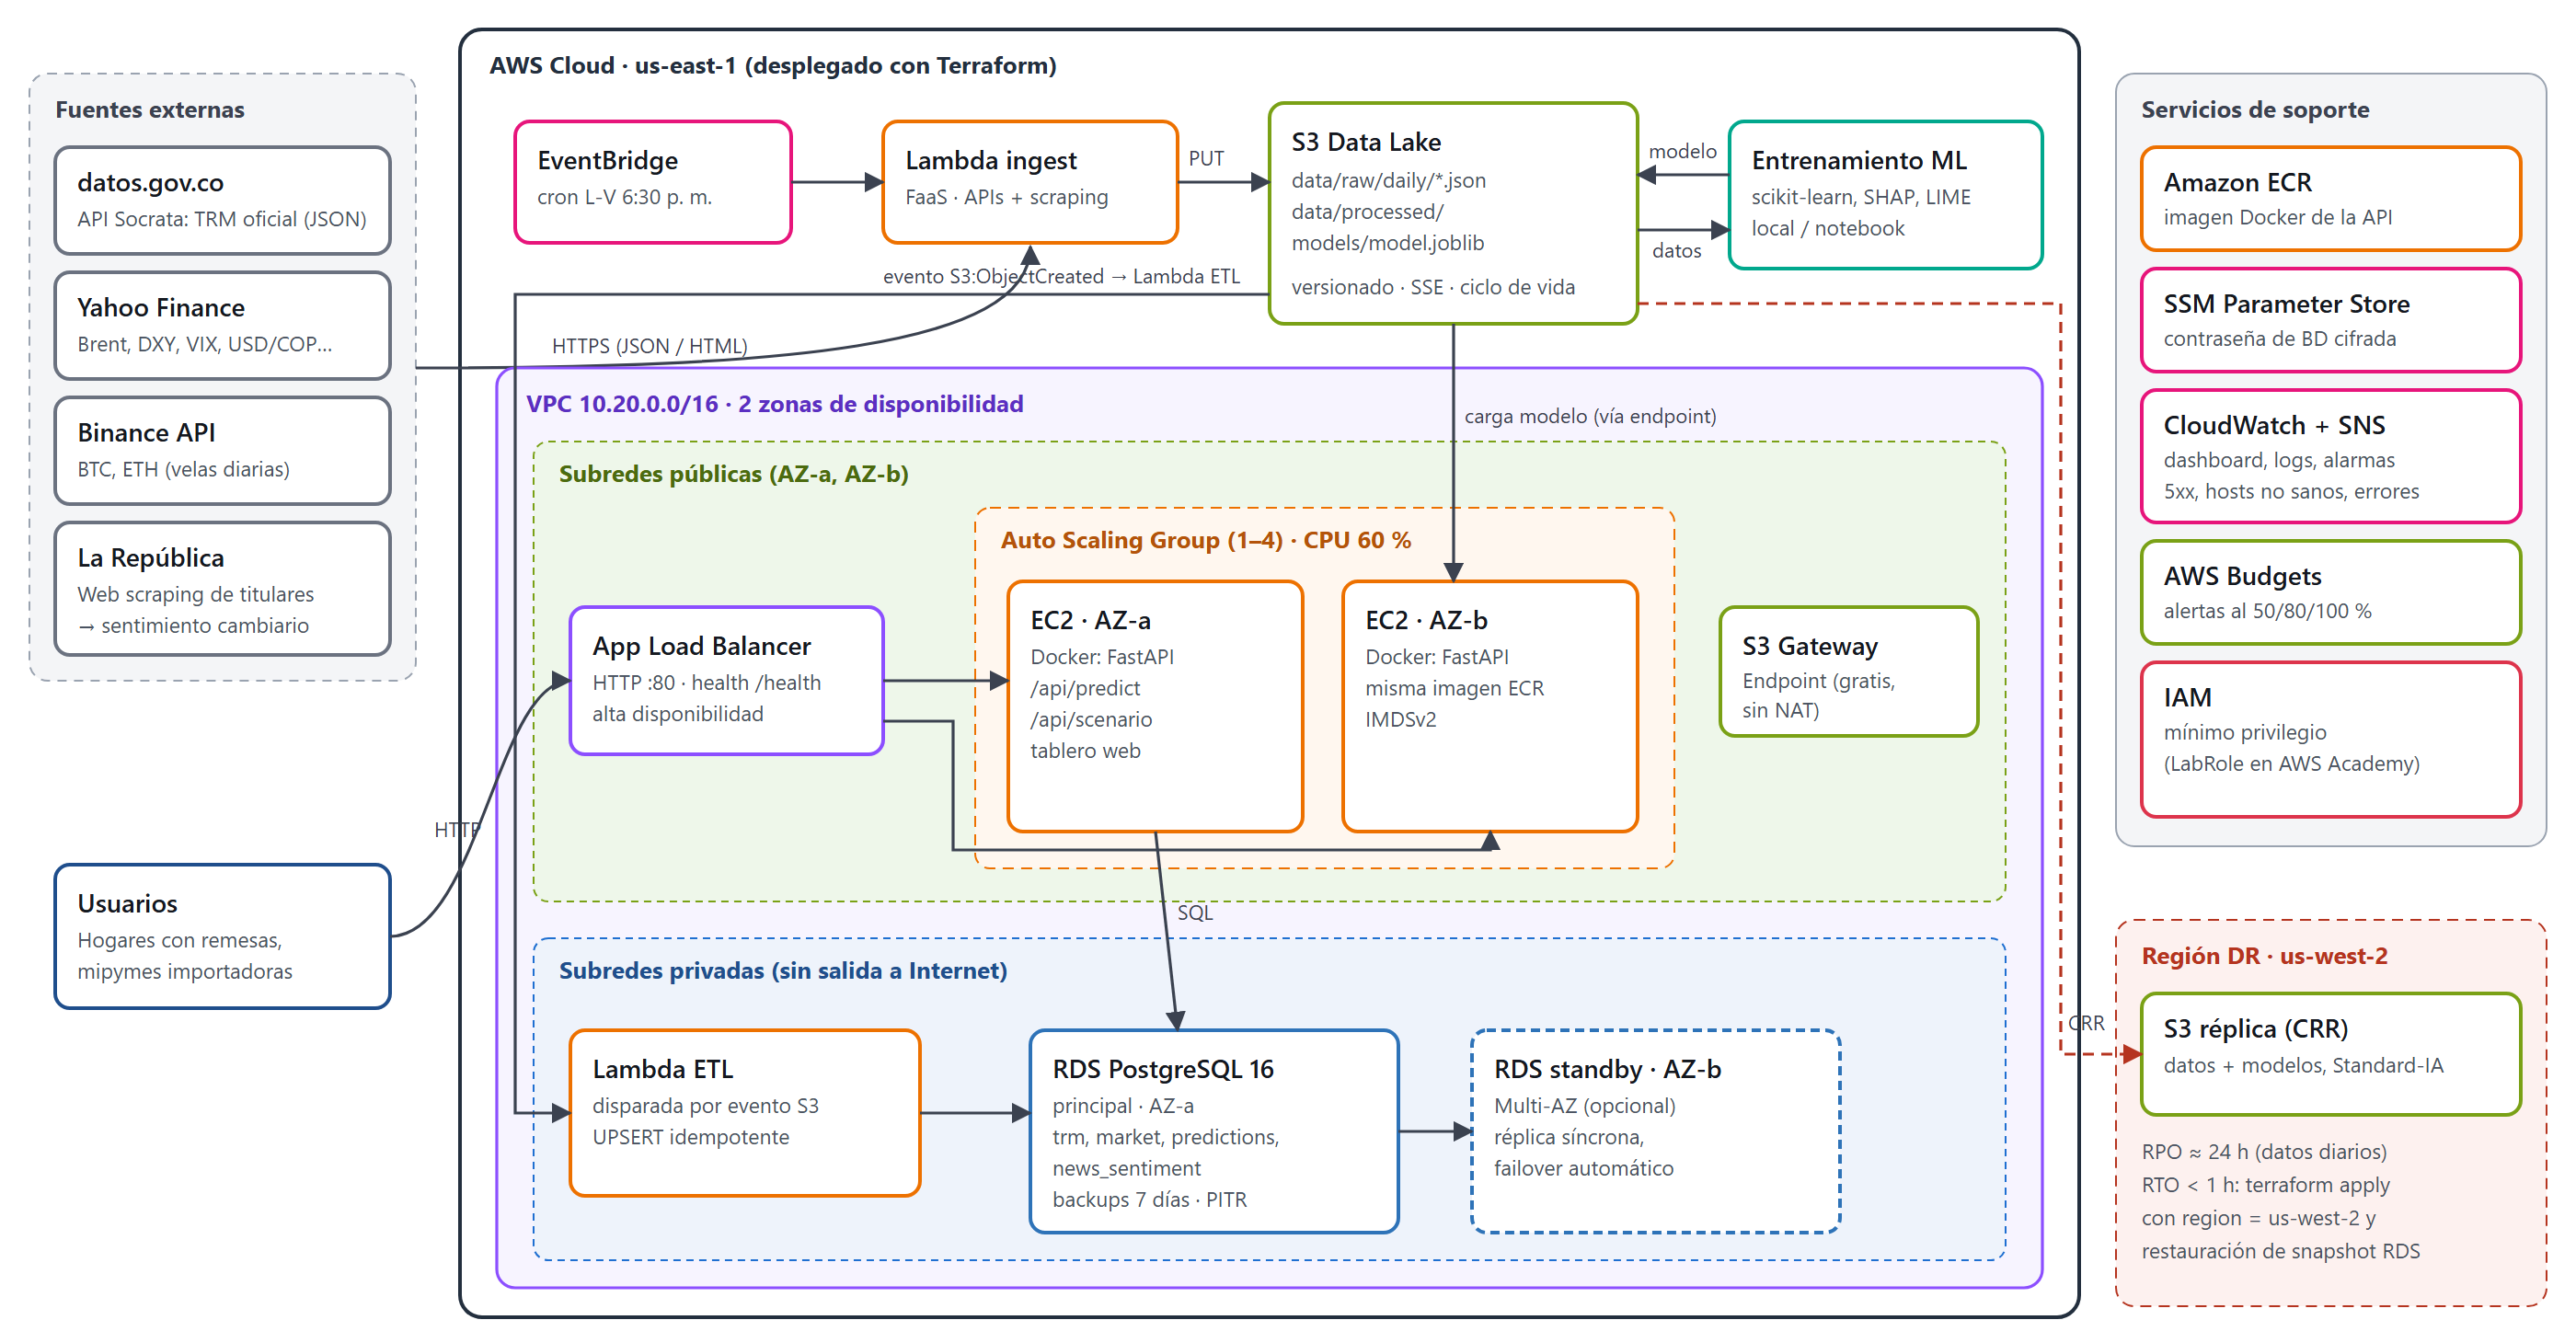
\includegraphics[width=0.95\textwidth]{arquitectura.png}
\caption{Arquitectura de TRM Predict en AWS, desplegada con Terraform.}
\label{fig:arch}
\end{figure*}

\section{Pipeline de minería de datos}
El pipeline sigue el proceso KDD~\cite{fayyad1996} organizado con CRISP-DM~\cite{wirth2000}; cada etapa es un módulo de Python que puede ejecutarse de principio a fin.

\subsection{Adquisición de datos}
La Tabla~\ref{tab:sources} resume las fuentes. El scraper cumple una función específica que ninguna API cubre: recoge los titulares de tres secciones de \emph{La República}, cuenta los que tratan del dólar y calcula un índice léxico de sentimiento cambiario (de $-1$ a $1$). Usa solo la librería estándar de Python para poder correr en Lambda, hace una petición por sección al día y aísla sus fallas de la ingesta numérica. Como no hay titulares históricos disponibles, el índice se almacena a diario y se muestra en el tablero; entrará a los modelos cuando acumule historia suficiente.

\begin{table}[t]
\caption{Fuentes de datos}
\label{tab:sources}
\centering
\footnotesize
\begin{tabular}{@{}p{2.1cm}p{1.4cm}p{3.9cm}@{}}
\toprule
Fuente & Formato & Contenido \\
\midrule
datos.gov.co (Superfinanciera) & API, JSON & TRM oficial desde 1991 (8.370 registros) \\
Yahoo Finance & API, JSON$\to$CSV & Brent, DXY, bono 10 años EE.~UU., VIX, S\&P 500, USD/MXN, USD/BRL, dólar spot USD/COP \\
Binance (data-api) & API, JSON$\to$CSV & Velas diarias de BTC y ETH \\
La República & Scraping HTML & Titulares e índice de sentimiento cambiario \\
\bottomrule
\end{tabular}
\end{table}

\subsection{Preparación y calidad de datos}
La limpieza incluye conversión de tipos, eliminación de duplicados y fechas inválidas, verificación de positividad y una auditoría de retornos atípicos con la regla de $3\times$IQR (por ejemplo, 61 en el Brent y 44 en el bono a 10 años; son eventos reales del mercado y se conservaron, pues los ensembles de árboles son robustos a ellos). La integración usa un \texttt{merge\_asof} estricto con \texttt{allow\_exact\_matches=False}: para la TRM vigente el día $d$ solo se usan cierres de mercado \emph{anteriores} a $d$, lo que evita la fuga de información futura. El conjunto final tiene 2.159 días (sep.~2017--oct.~2026), limitado por el inicio de las series de criptoactivos, y 43 variables (retornos logarítmicos y rezagos de la TRM, volatilidad a 5 y 20 días, razón de medias móviles, z-score, calendario; retornos a 1 y 5 días y volatilidad a 20 días de cada mercado; y la brecha spot--TRM). Los objetivos son el siguiente retorno logarítmico $y_{ret}$, su signo $y_{up}$ y un indicador de movimiento fuerte $y_{big}=\mathbb{1}[|y_{ret}|>q_{75}]$, con $q_{75}=0{,}86~\%$ calculado solo con el conjunto de entrenamiento.

\subsection{Análisis exploratorio}
Los retornos de la TRM son leptocúrticos (curtosis en exceso de 3,0; asimetría de 0,50; Jarque--Bera $p<10^{-100}$) y presentan autocorrelación positiva de primer orden (0,17), coherente con que la TRM es un promedio diario ponderado por volumen. Solo el 48,3~\% de los días son alzas. Las variables más correlacionadas con el siguiente retorno son el último retorno de la TRM (0,17), el Brent (0,13) y el DXY (0,09). Las correlaciones móviles (Fig.~\ref{fig:eda}) muestran que estas relaciones cambian de signo con el tiempo, lo que anticipa la baja predictibilidad fuera de muestra.

\begin{figure}[t]
\centering
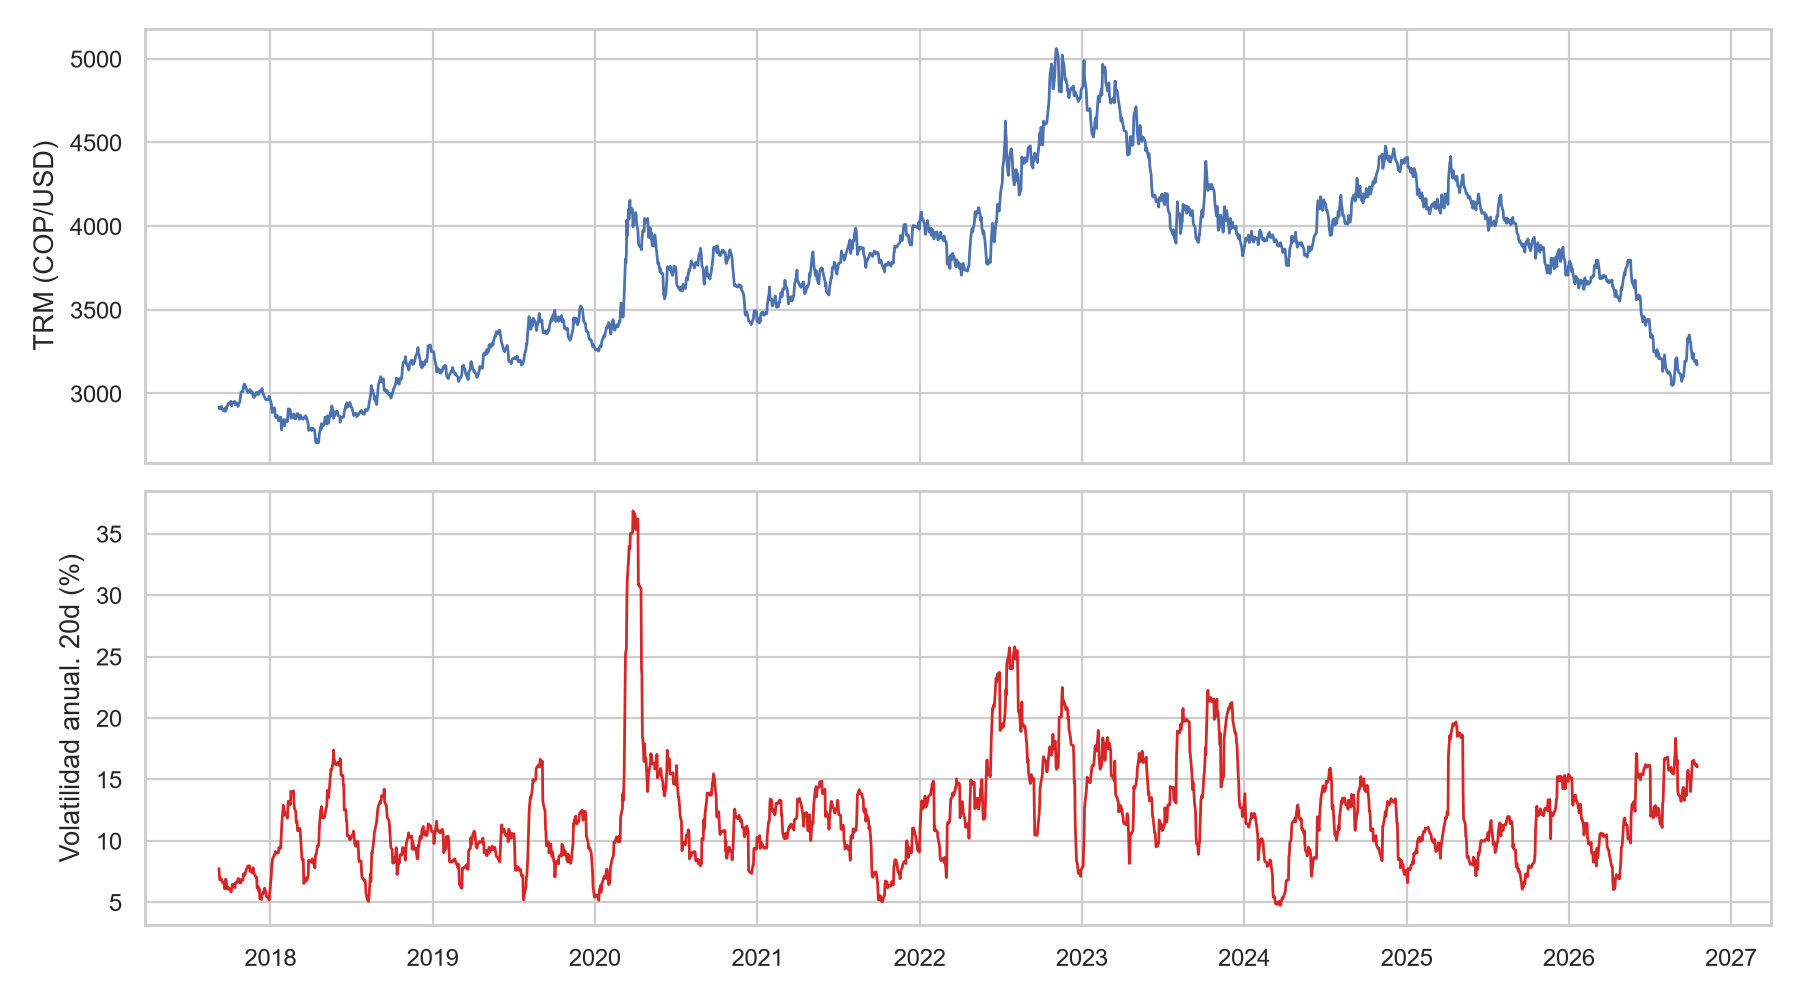
\includegraphics[width=\columnwidth]{eda_trm_series.png}\\[2pt]
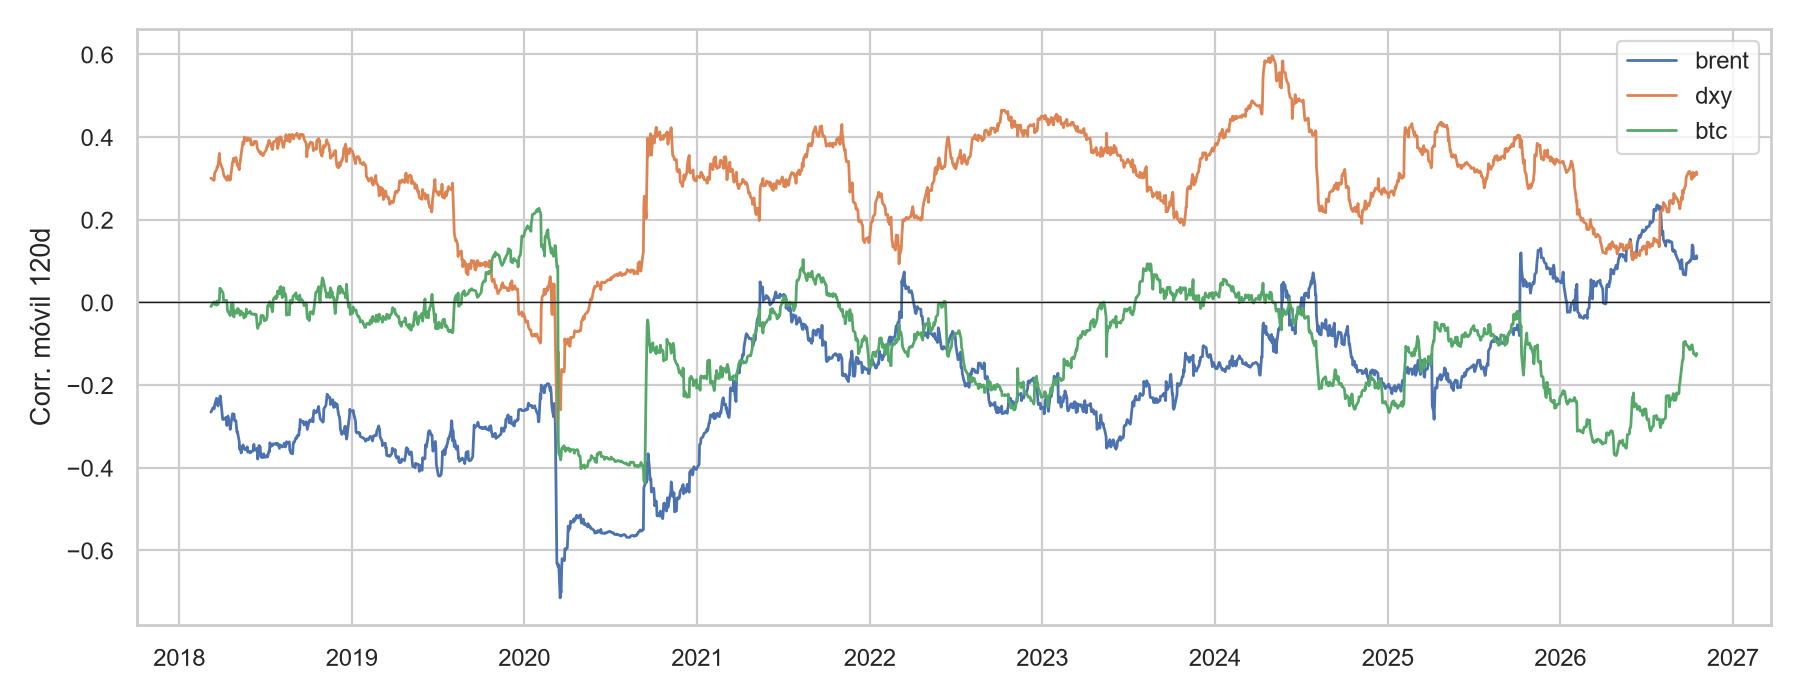
\includegraphics[width=\columnwidth]{eda_rolling_corr.png}
\caption{Nivel de la TRM y volatilidad anualizada a 20 días (arriba) y correlación móvil a 120 días entre la TRM y el Brent, el DXY y el BTC (abajo).}
\label{fig:eda}
\end{figure}

\subsection{Ingeniería de variables y PCA}
El PCA sobre las variables estandarizadas necesita 26 de 43 componentes para conservar el 90~\% de la varianza, así que las variables son poco redundantes y reducir dimensiones descartaría información; se usa solo para análisis y visualización. La PC1 carga en el momentum del peso y de las monedas pares (retorno a 5 días de la TRM, USD/COP, USD/MXN, z-score) y la PC2 en la volatilidad global (S\&P~500, bono a 10 años, Brent, DXY).

\subsection{Clustering: regímenes de mercado}
Se estandarizaron nueve variables de régimen (volatilidad y momentum a 5 días de la TRM, VIX, DXY, Brent, BTC y S\&P~500). Con los datos sin tratar, K-Means con $k=2$ solo aísla los 33 días más extremos de 2020; por eso las colas se recortaron a los percentiles 1--99 antes de aplicar K-Means y el clustering jerárquico de Ward, mientras que DBSCAN~\cite{ester1996} se aplicó sobre los datos sin recortar como detector de anomalías. El método de la silueta elige $k=3$ en ambos algoritmos (Tabla~\ref{tab:regimes}): un régimen de aversión al riesgo en el que la TRM sube el 52,9~\% de los días siguientes, uno de apetito por riesgo (44,3~\%) y uno de alta volatilidad, cuya volatilidad al día siguiente es 1,7 veces mayor. La silueta baja (0,12; Davies--Bouldin 2,08) indica regímenes traslapados, que por eso se usan como contexto y no como clases rígidas. DBSCAN ($\varepsilon=2{,}89$ a partir del percentil 95 de la curva de 18-distancias, \texttt{min\_samples}=18) marca 57 días anómalos (45 en 2020), en los que la volatilidad del día siguiente es 1,73 veces la de los días normales.

\begin{table}[t]
\caption{Regímenes de mercado de K-Means ($k=3$)}
\label{tab:regimes}
\centering
\footnotesize
\begin{tabular}{@{}lrrrr@{}}
\toprule
Régimen & Días & TRM sube & $\sigma$ ret. sig. & VIX 5d \\
\midrule
Aversión al riesgo & 972 & 52,9~\% & 0,78~\% & $+8{,}1$~\% \\
Alta volatilidad & 124 & 46,8~\% & 1,35~\% & $-1{,}7$~\% \\
Apetito por riesgo & 1.063 & 44,3~\% & 0,76~\% & $-6{,}7$~\% \\
\bottomrule
\end{tabular}
\end{table}

\subsection{Reglas de asociación}
Los retornos diarios de ocho mercados se discretizaron en terciles (\emph{sube}/\emph{baja}), junto con un indicador de alta volatilidad y la dirección de la siguiente TRM. Apriori~\cite{agrawal1994} y FP-Growth~\cite{han2000} (soporte mínimo 0,05; lift $\geq$ 1,05) producen los mismos 498 conjuntos frecuentes y 91 reglas cuyo consecuente es la dirección de la TRM, lo que valida ambas implementaciones entre sí. La Tabla~\ref{tab:rules} muestra las más fuertes, coherentes con la intuición económica: el petróleo al alza con un dólar global débil anticipa una apreciación del peso, y la depreciación conjunta de las monedas pares con un VIX al alza anticipa una subida de la TRM.

\begin{table}[t]
\caption{Reglas de asociación principales (FP-Growth)}
\label{tab:rules}
\centering
\footnotesize
\begin{tabular}{@{}p{3.6cm}p{0.9cm}rr@{}}
\toprule
Antecedente & TRM & Conf. & Lift \\
\midrule
BRL$\uparrow$, MXN$\uparrow$, VIX$\uparrow$ & sube & 0,60 & 1,24 \\
Brent$\uparrow$, S\&P$\uparrow$, VIX$\downarrow$ & baja & 0,64 & 1,24 \\
S\&P$\uparrow$, MXN$\uparrow$ & baja & 0,64 & 1,23 \\
Brent$\downarrow$, alta volatilidad & sube & 0,59 & 1,23 \\
DXY$\uparrow$, S\&P$\downarrow$, VIX$\uparrow$ & sube & 0,59 & 1,22 \\
Brent$\uparrow$, DXY$\downarrow$ & baja & 0,63 & 1,22 \\
\bottomrule
\end{tabular}
\end{table}

\section{Machine learning}
\subsection{Diseño experimental}
Los datos se dividieron cronológicamente: entrenamiento de sep.~2017 a dic.~2024 (1.727 días) y prueba de dic.~2024 a oct.~2026 (432 días). Dentro del entrenamiento, los hiperparámetros se optimizaron con \texttt{TimeSeriesSplit} de 5 pliegues, de modo que cada pliegue de validación queda después de su pliegue de entrenamiento. Todos los modelos son pipelines de scikit-learn~\cite{pedregosa2011}. Candidatos de regresión: lineal, polinomial (grado 2 sobre las $k$ mejores variables) + Ridge, Ridge, Lasso, Elastic Net, Random Forest~\cite{breiman2001} y Gradient Boosting~\cite{friedman2001}. Candidatos de clasificación (para dirección y riesgo): regresión logística, KNN, SVM (RBF), Random Forest, AdaBoost~\cite{freund1997} y Gradient Boosting. Se usó Grid Search en los espacios de baja dimensión (modelos lineales, KNN, SVM, AdaBoost) y Random Search~\cite{bergstra2012} con 15 muestras para los ensembles. Los modelos finales se eligen por el puntaje de validación cruzada, nunca por el de prueba.

\subsection{Resultados}
Las Tablas~\ref{tab:clf} y~\ref{tab:reg} reportan las métricas de prueba. En la clasificación de dirección, los modelos lineales, KNN y SVM quedan en el nivel del azar o por debajo (AUC 0,47--0,50), aunque su AUC en validación cruzada rondaba 0,56: su señal aparente no sobrevivió al cambio de periodo. Solo los ensembles conservan una ventaja (AUC 0,54--0,57), lo que indica interacciones no lineales entre los determinantes. El mismo patrón se observa en riesgo (AUC de hasta 0,586) y en regresión, donde Gradient Boosting reduce en 2,4~\% el RMSE del paseo aleatorio y Random Forest logra un acierto direccional del 54,6~\%. La exactitud en dirección con umbral 0,5 (53,2~\%) aún está por debajo de la clase mayoritaria (54,6~\%, un periodo en el que el peso se apreció), limitación que se discute en la Sección~\ref{sec:disc}.

\begin{table}[t]
\caption{Resultados de prueba: clasificación (432 días)}
\label{tab:clf}
\centering
\footnotesize
\begin{tabular}{@{}lccccc@{}}
\toprule
 & \multicolumn{3}{c}{Dirección} & \multicolumn{2}{c}{Riesgo} \\
\cmidrule(lr){2-4}\cmidrule(l){5-6}
Modelo & AUC VC & AUC & Exact. & AUC VC & AUC \\
\midrule
Logística & 0,559 & 0,497 & 0,519 & 0,599 & 0,549 \\
KNN & 0,565 & 0,474 & 0,486 & 0,597 & 0,571 \\
SVM & 0,557 & 0,490 & 0,484 & 0,595 & 0,562 \\
Random Forest & \textbf{0,582} & 0,555 & 0,532 & \textbf{0,623} & 0,585 \\
AdaBoost & 0,562 & 0,541 & 0,521 & 0,600 & 0,557 \\
Gradient Boost. & 0,578 & \textbf{0,566} & 0,532 & 0,615 & \textbf{0,586} \\
\midrule
Línea base & -- & 0,500 & 0,546 & -- & 0,500 \\
\bottomrule
\end{tabular}
\end{table}

\begin{table}[t]
\caption{Resultados de prueba: regresión del siguiente retorno}
\label{tab:reg}
\centering
\footnotesize
\begin{tabular}{@{}lcccc@{}}
\toprule
Modelo & RMSE (\%) & RMSE/PA & $R^2$ & Acierto dir. \\
\midrule
Paseo aleatorio & 0,769 & 1,000 & -- & -- \\
Lineal & 0,772 & 1,005 & $-0{,}019$ & 0,509 \\
Poli(2)+Ridge & 0,764 & 0,993 & 0,004 & 0,500 \\
Ridge & 0,767 & 0,997 & $-0{,}004$ & 0,493 \\
Lasso & 0,765 & 0,995 & 0,000 & 0,502 \\
Elastic Net & 0,765 & 0,994 & 0,002 & 0,491 \\
Random Forest & 0,759 & 0,987 & 0,017 & \textbf{0,546} \\
Gradient Boost. & \textbf{0,751} & \textbf{0,976} & \textbf{0,038} & 0,542 \\
\bottomrule
\end{tabular}
\end{table}

\subsection{Interpretabilidad}
TreeSHAP sobre el modelo de dirección Random Forest (Fig.~\ref{fig:shap}) ubica en primer lugar la brecha spot--TRM: cuando la última cotización spot está por encima de la TRM vigente, la siguiente TRM tiende a subir, lo que refleja que la TRM promedia las operaciones del día. Le siguen el último retorno de la TRM, la variación diaria del DXY y del dólar spot y el retorno a 5 días del Brent. La importancia por impureza coincide en cuatro de las cinco primeras variables (brecha spot--TRM, último retorno de la TRM y variaciones diarias del USD/COP y del DXY). LIME sobre el último día de prueba da una explicación local: el alza del 5~\% del Brent en cinco días y la caída del 1~\% del dólar spot el día anterior reducen la probabilidad de alza, mientras que la brecha spot--TRM y el último retorno de la TRM la aumentan. Es una explicación legible que puede mostrarse junto a cada pronóstico.

\begin{figure}[t]
\centering
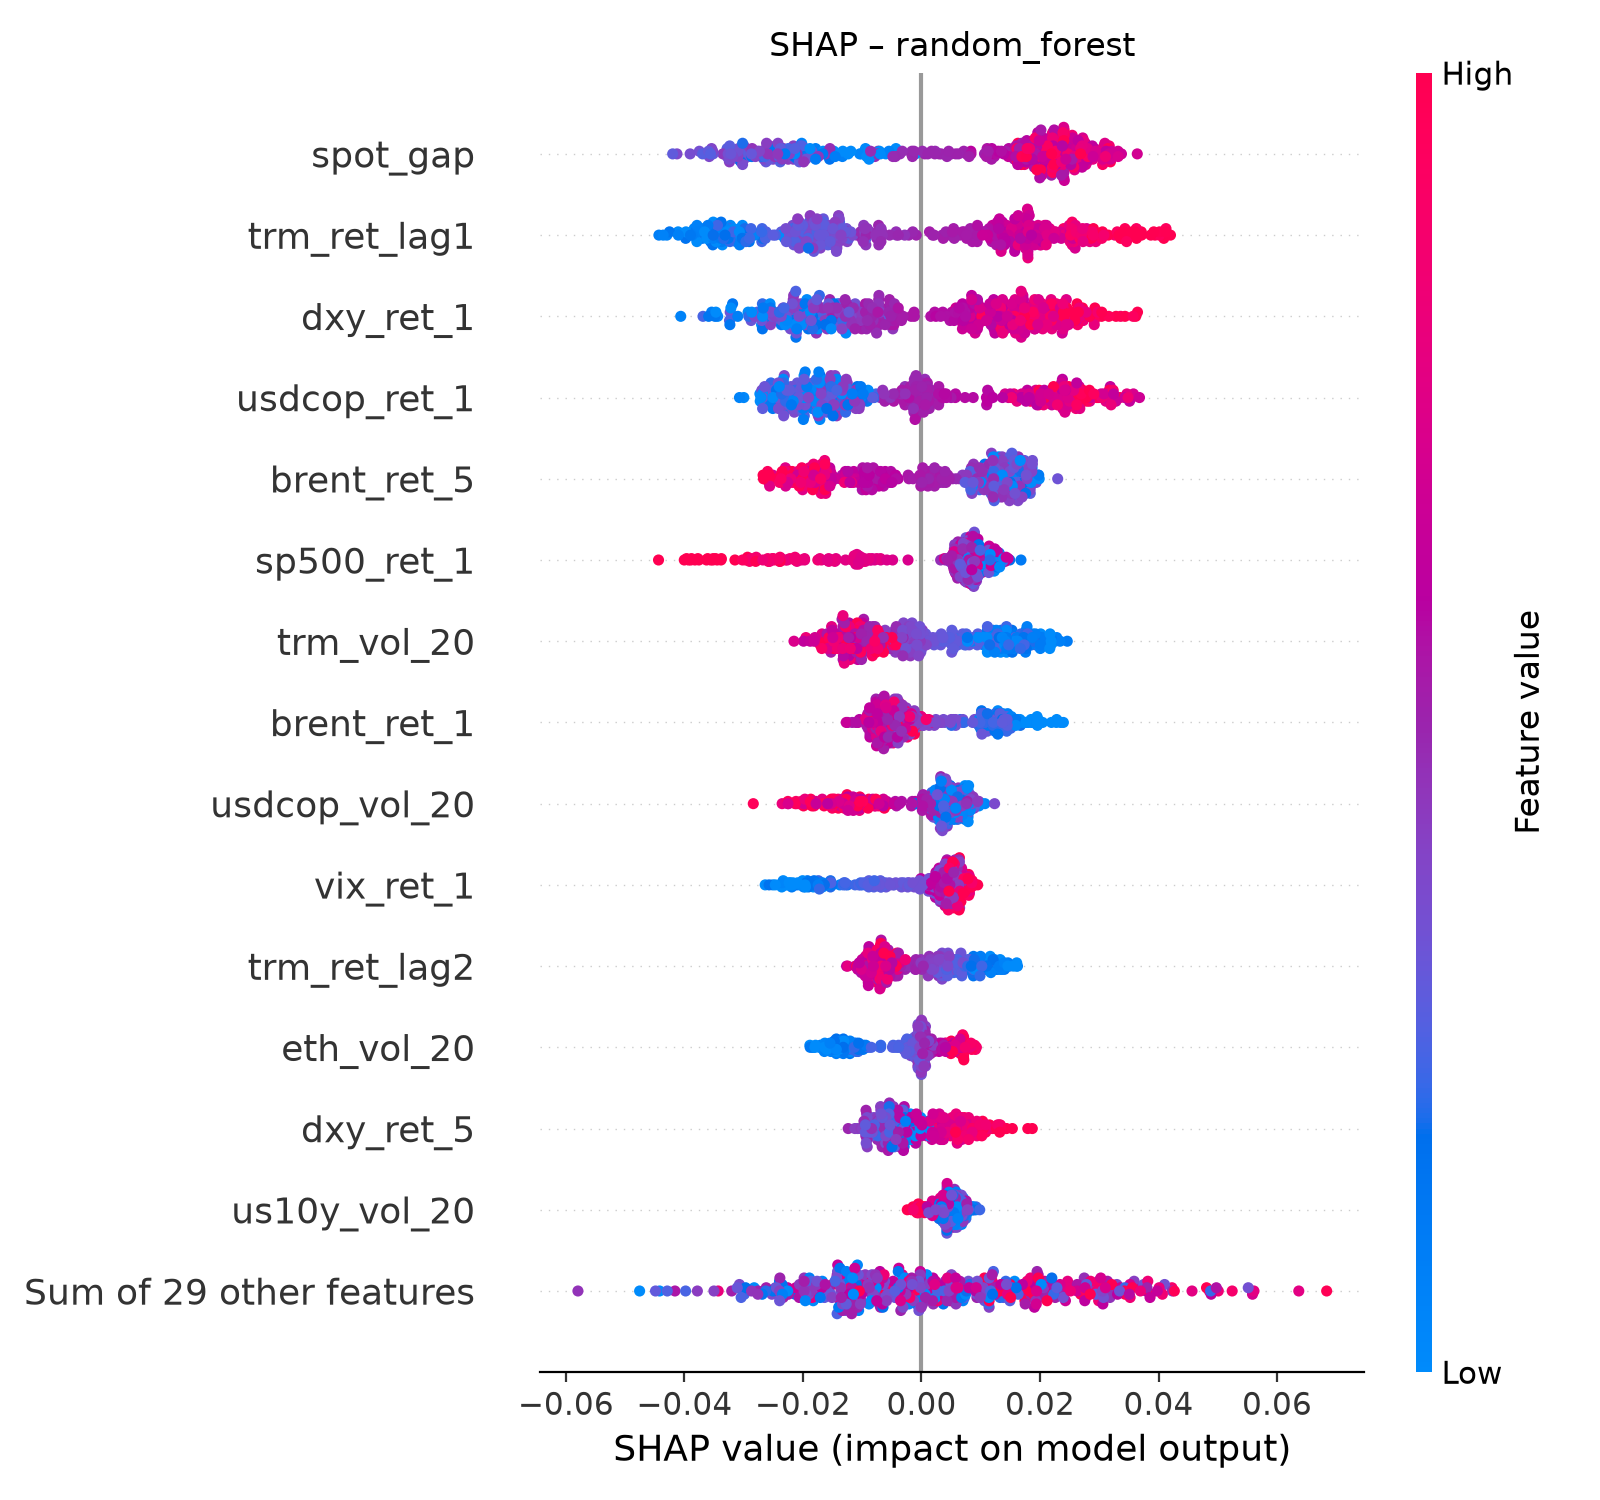
\includegraphics[width=0.92\columnwidth]{shap_beeswarm.png}
\caption{Valores SHAP del modelo de dirección Random Forest en el conjunto de prueba.}
\label{fig:shap}
\end{figure}

\subsection{Evaluación orientada a decisiones}
Las métricas estadísticas no dicen si el modelo ayuda a un usuario. Simulamos un hogar que recibe USD~1.000 al día y vende a la TRM vigente, o espera un día cuando $P(\text{sube})>\tau$. En el periodo de prueba (Fig.~\ref{fig:backtest}), la regla con Random Forest y $\tau=0{,}5$ gana en promedio 383 COP al día frente a vender siempre de inmediato, y 624 COP con $\tau=0{,}55$; con Gradient Boosting gana 495 y 1.832 COP, respectivamente. Decidir al azar entre vender o esperar \emph{pierde} 1.383 COP al día, porque el peso se apreció durante el periodo de prueba, y un oráculo perfecto ganaría 9.994 COP. Las ganancias son pequeñas pero positivas y robustas al umbral. Para la alerta de riesgo, un umbral de probabilidad elegido en el último pliegue de entrenamiento, de modo que la tasa de alertas iguale la frecuencia histórica, logra en prueba una precisión del 30,1~\% frente a una tasa base del 22,5~\% (lift 1,34), con una exhaustividad del 25,8~\%. Las probabilidades del Random Forest están algo mejor calibradas que la tasa base (Brier 0,247 frente a 0,249).

\begin{figure}[t]
\centering
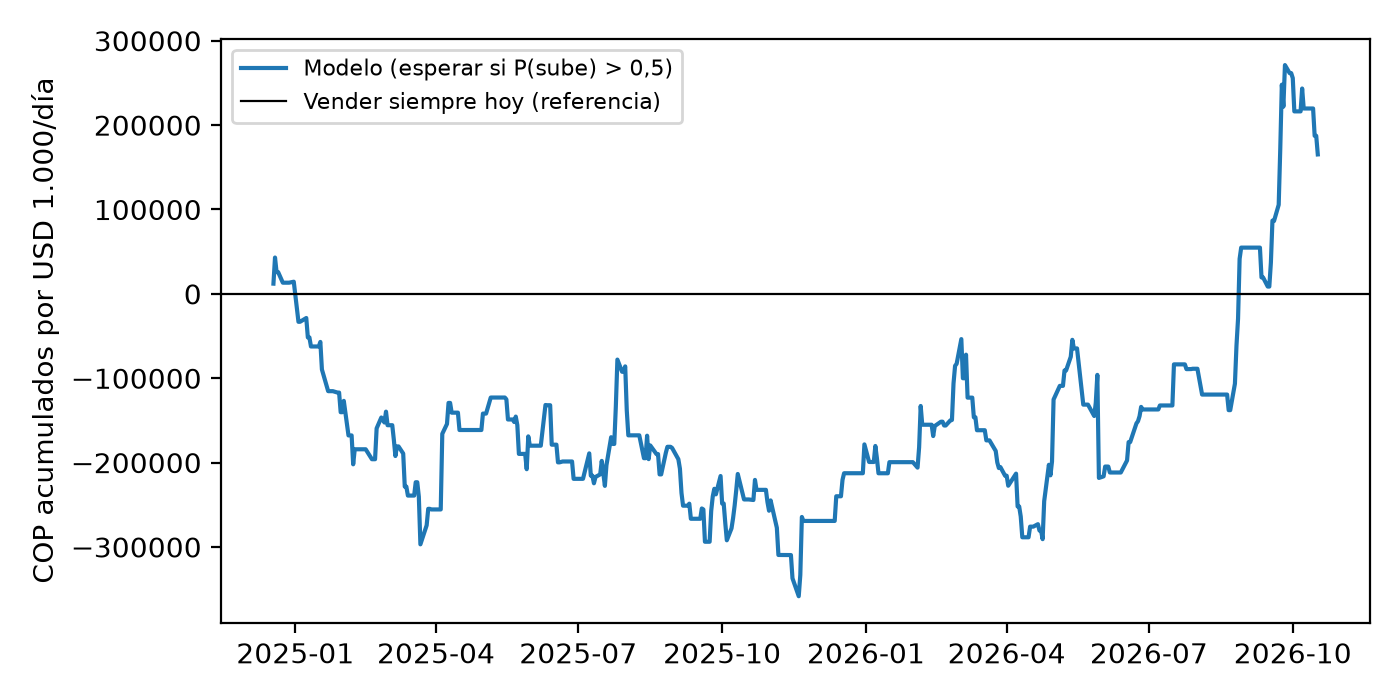
\includegraphics[width=\columnwidth]{decision_backtest.png}
\caption{Ganancia acumulada de la regla del hogar con remesas (Random Forest, $\tau=0{,}5$) frente a vender siempre de inmediato.}
\label{fig:backtest}
\end{figure}

\subsection{Selección del modelo}
Se eligió Random Forest para dirección, riesgo y regresión porque obtiene el mejor puntaje de validación cruzada en dos de las tres tareas, nunca queda lejos del mejor resultado de prueba y una sola familia de modelos simplifica el mantenimiento y la explicación. La búsqueda aleatoria de cada ensemble tarda de 60 a 77~s en un portátil, y servir los tres modelos toma cerca de 0,5~s por petición en una \texttt{t3.micro}. Gradient Boosting se conserva como alternativa documentada, pues obtuvo puntajes de prueba ligeramente mejores.

\section{Arquitectura y despliegue en la nube}
\subsection{Modelos de servicio y de despliegue}
El sistema usa la nube pública de AWS (us-east-1) y una segunda región (us-west-2) para recuperación ante desastres. Siguiendo al NIST~\cite{nist800145}, combina cuatro modelos de servicio (Tabla~\ref{tab:services}), cada uno con una razón: FaaS donde el trabajo es esporádico, PaaS donde hay que gestionar estado e IaaS donde el curso exige control explícito del balanceo de carga y el auto-scaling.

\begin{table}[t]
\caption{Modelos de servicio y justificación}
\label{tab:services}
\centering
\footnotesize
\begin{tabular}{@{}p{1.0cm}p{2.3cm}p{4.1cm}@{}}
\toprule
Modelo & Servicio & Por qué \\
\midrule
FaaS & Lambda + EventBridge & La ingesta y el ETL corren segundos al día; pagar por invocación es casi gratis \\
PaaS & RDS PostgreSQL & Backups, parches y failover Multi-AZ administrados \\
PaaS & S3, ECR, ALB & Data lake durable, registro de imágenes y balanceo administrado \\
IaaS & EC2 + Auto Scaling & Control explícito del tipo de instancia, la política de escalado y los health checks \\
SaaS & Tablero web & Lo consumen los usuarios finales desde el navegador \\
\bottomrule
\end{tabular}
\end{table}

\subsection{Infraestructura como código}
Toda la infraestructura está declarada en Terraform~\cite{terraform_aws} (10 archivos, 64 recursos administrados): VPC con subredes públicas y privadas en dos zonas de disponibilidad, security groups, un endpoint gateway de S3 gratuito que reemplaza un NAT gateway, el data lake versionado y cifrado con reglas de ciclo de vida, réplica entre regiones, ECR, RDS, parámetros de SSM, ALB, launch template, Auto Scaling Group y política target tracking, las dos Lambdas con sus disparadores, alarmas y tablero de CloudWatch y un presupuesto mensual de AWS Budgets. Un solo \texttt{terraform apply} crea la plataforma en unos 15 minutos, la mayoría para RDS, y \texttt{terraform destroy} la elimina. Las variables permiten ejecutar el mismo código en AWS Academy, cuyo \texttt{LabRole} reemplaza los roles IAM que Terraform crearía en otro caso.

\subsection{Seguridad}
RDS y la Lambda de ETL están en subredes privadas sin salida a Internet; la base de datos solo acepta conexiones de los security groups de la API y del ETL; las instancias de la API solo aceptan tráfico del ALB y exigen IMDSv2; la contraseña de la base de datos la genera Terraform y se guarda cifrada en SSM Parameter Store; S3 bloquea el acceso público y cifra en reposo. No se procesan datos personales, por lo que no se requiere consentimiento informado.

\subsection{Escalabilidad y alta disponibilidad: experimentos}
Se hicieron dos experimentos sobre la plataforma desplegada desde un cliente en Colombia (Tabla~\ref{tab:exp}). Sin carga, \texttt{/health} responde en 197~ms (casi todo es la ida y vuelta por la red), \texttt{/api/predict} en 709~ms y \texttt{/api/scenario} en 982~ms.

\emph{Alta disponibilidad.} Una sonda consultó \texttt{/health} cada 0,5~s y se terminó una instancia en $t=30$~s (Fig.~\ref{fig:ha}). En la primera corrida el grupo de auto-scaling tenía un mínimo de una instancia: como el grupo inactivo ya se había reducido a un solo servidor, terminarlo dejó al balanceador sin destinos durante unos 109~s, hasta que el reemplazo pasó los chequeos de salud (disponibilidad de 77,8~\%). Al subir el mínimo a dos (una por zona), la misma prueba dio 378 peticiones exitosas de 378; el balanceador retiró el destino caído y el grupo recuperó la capacidad completa en 139~s. La lección es que la alta disponibilidad depende tanto de la política de escalado como de la topología multi-AZ.

\emph{Escalabilidad.} Dieciséis clientes concurrentes enviaron peticiones \texttt{POST /api/scenario}, el endpoint que más CPU consume, durante 14~min (Fig.~\ref{fig:load}). El target tracking al 60~\% de CPU subió la capacidad deseada de dos a cuatro en el minuto 6,6, y las nuevas instancias quedaron sanas en el minuto 9,2. El rendimiento pasó de 4,1 a 7,6 peticiones/s (+84~\%) y la latencia mediana bajó de 4,0 a 1,6~s, sin errores en 4.543 peticiones. Los cerca de 2,5~min entre la decisión de escalar y la nueva capacidad se deben sobre todo al arranque de la instancia y a la descarga de la imagen, que un warm pool o una imagen más liviana acortarían.

\begin{table}[t]
\caption{Resultados de los experimentos en la nube}
\label{tab:exp}
\centering
\footnotesize
\begin{tabular}{@{}lrrr@{}}
\toprule
\multicolumn{4}{@{}l}{\emph{Alta disponibilidad (se termina una instancia)}} \\
Mínimo del ASG & Disponib. & Caída & Recuperación \\
\midrule
1 instancia & 77,8~\% & 109~s & --- \\
2 instancias & 100~\% & 0~s & 139~s \\
\midrule
\multicolumn{4}{@{}l}{\emph{Prueba de carga (16 clientes, 4.543 peticiones, 0 errores)}} \\
Instancias & Pet./s & p50 (s) & p95 (s) \\
\midrule
2 & 4,12 & 4,05 & 7,62 \\
4 & 7,59 & 1,61 & 4,87 \\
\bottomrule
\end{tabular}
\end{table}

\begin{figure}[t]
\centering
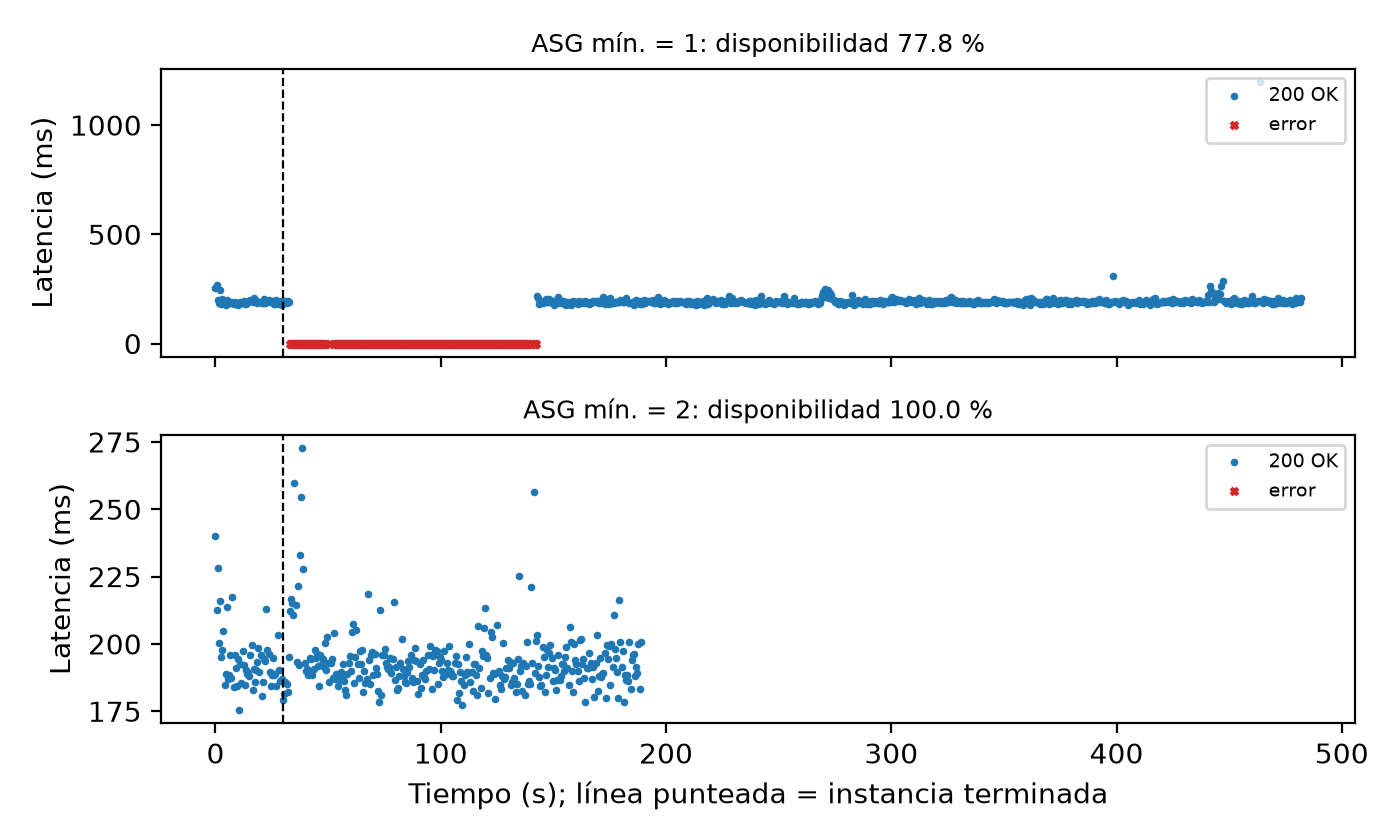
\includegraphics[width=\columnwidth]{ha_timeline.png}
\caption{Latencia de las sondas a \texttt{/health} al terminar una instancia (línea punteada) con un mínimo de una (arriba) y de dos instancias (abajo). Las cruces rojas son peticiones fallidas.}
\label{fig:ha}
\end{figure}

\begin{figure}[t]
\centering
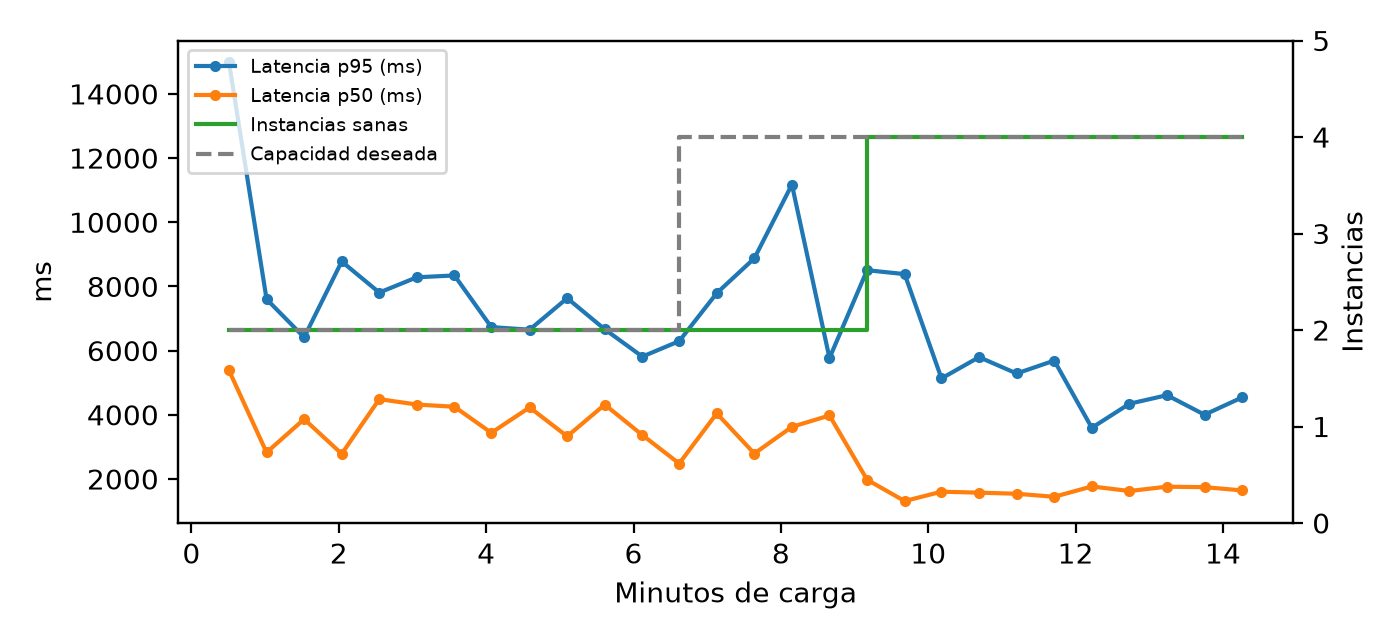
\includegraphics[width=\columnwidth]{load_timeline.png}
\caption{Prueba de carga: latencia p50 y p95, capacidad deseada e instancias sanas. La latencia baja cuando las dos nuevas instancias pasan los chequeos de salud.}
\label{fig:load}
\end{figure}

\subsection{Recuperación ante desastres}
El versionado de S3 protege contra borrados accidentales, y la réplica entre regiones copió a us-west-2, en cuestión de minutos, el paquete histórico de 1,6~MB y el modelo de 12~MB. RDS conserva siete días de backups automáticos con recuperación a un punto en el tiempo. Como todos los datos pueden volver a obtenerse de fuentes públicas y toda la infraestructura es código, la estrategia es \emph{backup and restore}~\cite{aws_wellarchitected}, con RPO $\approx$ 24~h y RTO $<$ 1~h: \texttt{terraform apply} con \texttt{region=us-west-2} recrea la plataforma y la carga histórica vuelve a poblar la base de datos en unos 2 minutos (14~s de ingesta y 109~s de ETL medidos).

\subsection{Análisis de costos}
La Tabla~\ref{tab:cost} compara el estimado on-demand con el uso observado. Los costos dominantes son el ALB, las direcciones IPv4 públicas y las instancias de EC2 y RDS siempre encendidas; S3, Lambda, EventBridge y SSM son despreciables. Evitar el NAT gateway ahorra unos USD~33 al mes. Como la plataforma se crea y se destruye con Terraform, el costo esperado de todo el semestre (unas 40 horas de desarrollo, un día de pruebas y una semana de operación para la sustentación) es de unos USD~21. El despliegue usado para los experimentos estuvo activo unos dos días, a un costo estimado de USD~2 diarios; AWS Cost Explorer reporta los cargos con unas 24~h de retraso, por lo que el valor facturado se agrega al repositorio (\texttt{docs/costos.md}) cuando se consolide.

\begin{table}[t]
\caption{Costo mensual estimado (USD, on-demand, us-east-1, 24/7)}
\label{tab:cost}
\centering
\footnotesize
\begin{tabular}{@{}lr@{}}
\toprule
Servicio (configuración) & USD/mes \\
\midrule
Application Load Balancer (tráfico bajo) & 17,0 \\
EC2: 2 $\times$ t3.micro + 16 GB gp3 & 16,5 \\
Direcciones IPv4 públicas (4) & 14,6 \\
RDS PostgreSQL db.t4g.micro + 20 GB & 14,0 \\
S3 + réplica entre regiones, ECR & 0,2 \\
Lambda, EventBridge, SSM & 0,0 \\
CloudWatch, transferencia de datos & 1,3 \\
\midrule
\textbf{Total (dev, Single-AZ)} & \textbf{63,6} \\
Producción (Multi-AZ, hasta 4 instancias) & 78--95 \\
Alternativa serverless (API Gateway + Lambda) & $<$ 5 \\
\bottomrule
\end{tabular}
\end{table}

\section{Integración y demostración}
\begin{figure}[t]
\centering
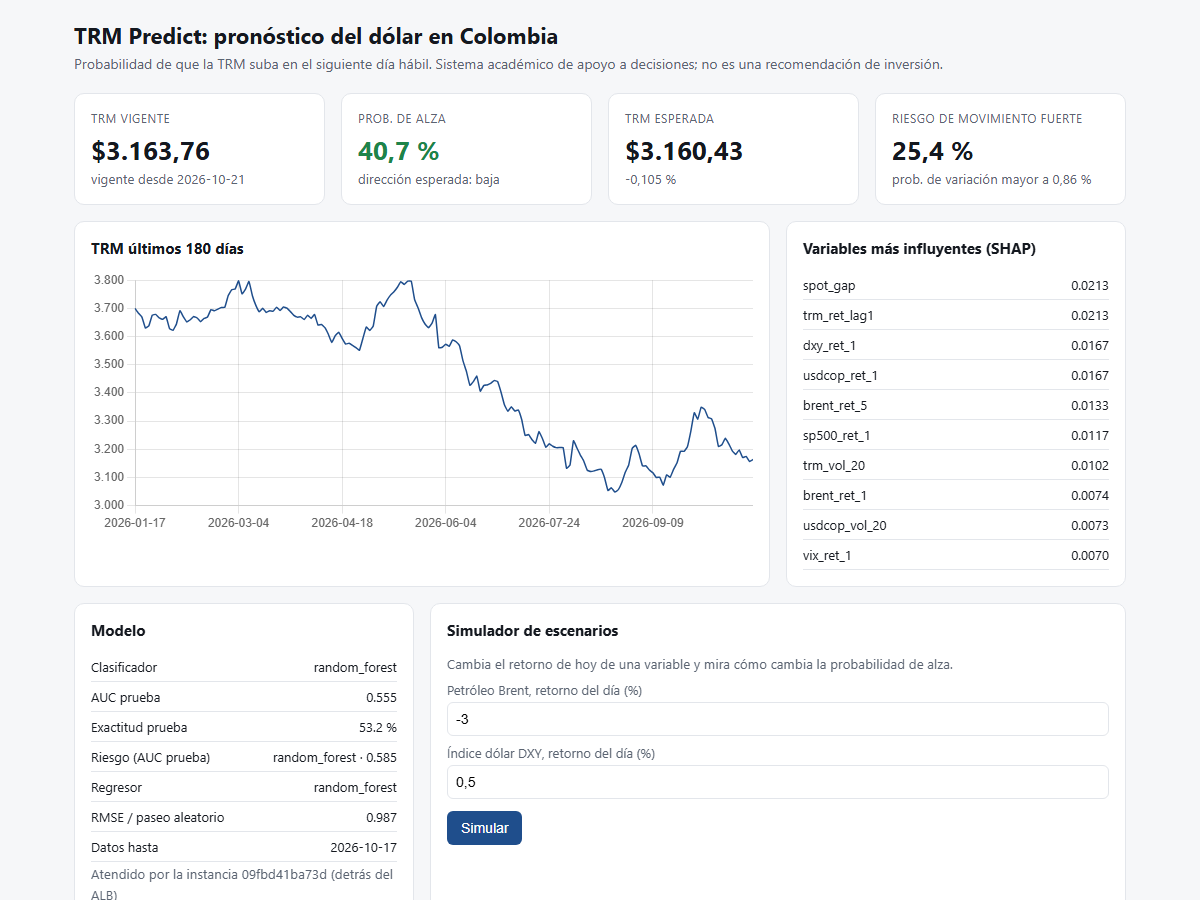
\includegraphics[width=\columnwidth]{tablero_aws.png}
\caption{Tablero servido desde AWS: TRM vigente, probabilidad de alza, TRM esperada, riesgo de movimiento fuerte, variables SHAP y simulador de escenarios.}
\label{fig:dash}
\end{figure}

El sistema desplegado funciona de punta a punta: la carga histórica llevó a RDS 2.321 registros de TRM y 26.682 observaciones de mercado, la programación diaria los actualiza después de cada publicación, y el tablero (Fig.~\ref{fig:dash}) y la API REST (\texttt{/api/predict}, \texttt{/api/scenario}, \texttt{/api/history}, \texttt{/api/model}) responden desde ambas zonas de disponibilidad. El \emph{simulador de escenarios} permite preguntar, por ejemplo, cómo cambia la probabilidad de alza si el petróleo cae 3~\% y el DXY sube 0,5~\%. El código, el conjunto de datos, el modelo entrenado y los scripts de Terraform están en el repositorio público~\cite{repo}.

\section{Discusión y limitaciones}
\label{sec:disc}
Los resultados confirman la dificultad documentada desde Meese y Rogoff~\cite{meese1983}: el componente predecible de los movimientos cambiarios diarios es pequeño e inestable. De ahí salen tres lecciones. Primera, la validación cruzada por sí sola fue engañosa: todos los modelos tenían un AUC de validación cercano a 0,56--0,58, pero solo los ensembles conservaron una ventaja en un periodo posterior no visto; un conjunto de prueba estrictamente cronológico fue indispensable. Segunda, la variable más útil (brecha spot--TRM) proviene de entender cómo se calcula la TRM, no de la complejidad del modelo. Tercera, las métricas orientadas a decisiones hacen interpretables para el usuario ganancias estadísticas modestas. Limitaciones: el periodo de prueba estuvo dominado por la apreciación del peso, por lo que la exactitud con umbral 0,5 está por debajo de la clase mayoritaria; el índice de sentimiento aún no tiene historia; Yahoo Finance es una fuente no oficial; y el inicio en 2017 de los datos de criptoactivos acorta la muestra.

\section{Conclusiones y trabajo futuro}
TRM Predict integra en un solo producto, alineado con los ODS 8 y 10, un pipeline completo de minería de datos, un conjunto de modelos de machine learning evaluados con honestidad y una arquitectura escalable y de alta disponibilidad en AWS definida como código. Los ensembles fueron los únicos modelos con valor fuera de muestra, y su señal se traduce en ganancias pequeñas pero positivas para un hogar con remesas. Trabajo futuro: calibración de probabilidades y umbrales sensibles al costo, incorporar el índice de sentimiento acumulado y el diferencial de tasas de política monetaria, reentrenamiento walk-forward programado en la nube y una versión serverless de la API para reducir el costo a menos de USD~5 al mes.

\begin{thebibliography}{99}
\bibitem{banrep_remesas} Banco de la Rep\'ublica de Colombia, ``Ingresos de remesas de trabajadores en Colombia,'' Estad\'isticas del sector externo, 2025. [En línea]. Disponible: \url{https://www.banrep.gov.co}
\bibitem{un2015} United Nations, ``Transforming our world: The 2030 Agenda for Sustainable Development,'' A/RES/70/1, 2015.
\bibitem{meese1983} R. A. Meese and K. Rogoff, ``Empirical exchange rate models of the seventies: Do they fit out of sample?'' \emph{J. Int. Econ.}, vol. 14, no. 1--2, pp. 3--24, 1983.
\bibitem{henrique2019} B. M. Henrique, V. A. Sobreiro, and H. Kimura, ``Literature review: Machine learning techniques applied to financial market prediction,'' \emph{Expert Syst. Appl.}, vol. 124, pp. 226--251, 2019.
\bibitem{sezer2020} O. B. Sezer, M. U. Gudelek, and A. M. Ozbayoglu, ``Financial time series forecasting with deep learning: A systematic literature review: 2005--2019,'' \emph{Appl. Soft Comput.}, vol. 90, Art. no. 106181, 2020.
\bibitem{lundberg2017} S. M. Lundberg and S.-I. Lee, ``A unified approach to interpreting model predictions,'' in \emph{Adv. Neural Inf. Process. Syst. (NeurIPS)}, vol. 30, 2017, pp. 4765--4774.
\bibitem{ribeiro2016} M. T. Ribeiro, S. Singh, and C. Guestrin, ```Why should I trust you?': Explaining the predictions of any classifier,'' in \emph{Proc. 22nd ACM SIGKDD Int. Conf. Knowl. Discov. Data Min.}, 2016, pp. 1135--1144.
\bibitem{fayyad1996} U. Fayyad, G. Piatetsky-Shapiro, and P. Smyth, ``From data mining to knowledge discovery in databases,'' \emph{AI Mag.}, vol. 17, no. 3, pp. 37--54, 1996.
\bibitem{wirth2000} R. Wirth and J. Hipp, ``CRISP-DM: Towards a standard process model for data mining,'' in \emph{Proc. 4th Int. Conf. Pract. Appl. Knowl. Discov. Data Min.}, 2000, pp. 29--39.
\bibitem{ester1996} M. Ester, H.-P. Kriegel, J. Sander, and X. Xu, ``A density-based algorithm for discovering clusters in large spatial databases with noise,'' in \emph{Proc. 2nd Int. Conf. Knowl. Discov. Data Min. (KDD)}, 1996, pp. 226--231.
\bibitem{agrawal1994} R. Agrawal and R. Srikant, ``Fast algorithms for mining association rules,'' in \emph{Proc. 20th Int. Conf. Very Large Data Bases (VLDB)}, 1994, pp. 487--499.
\bibitem{han2000} J. Han, J. Pei, and Y. Yin, ``Mining frequent patterns without candidate generation,'' in \emph{Proc. ACM SIGMOD Int. Conf. Manag. Data}, 2000, pp. 1--12.
\bibitem{pedregosa2011} F. Pedregosa \emph{et al.}, ``Scikit-learn: Machine learning in Python,'' \emph{J. Mach. Learn. Res.}, vol. 12, pp. 2825--2830, 2011.
\bibitem{breiman2001} L. Breiman, ``Random forests,'' \emph{Mach. Learn.}, vol. 45, no. 1, pp. 5--32, 2001.
\bibitem{friedman2001} J. H. Friedman, ``Greedy function approximation: A gradient boosting machine,'' \emph{Ann. Statist.}, vol. 29, no. 5, pp. 1189--1232, 2001.
\bibitem{freund1997} Y. Freund and R. E. Schapire, ``A decision-theoretic generalization of on-line learning and an application to boosting,'' \emph{J. Comput. Syst. Sci.}, vol. 55, no. 1, pp. 119--139, 1997.
\bibitem{bergstra2012} J. Bergstra and Y. Bengio, ``Random search for hyper-parameter optimization,'' \emph{J. Mach. Learn. Res.}, vol. 13, pp. 281--305, 2012.
\bibitem{nist800145} P. Mell and T. Grance, ``The NIST definition of cloud computing,'' NIST, Gaithersburg, MD, USA, Special Publication 800-145, 2011.
\bibitem{terraform_aws} HashiCorp, ``Terraform AWS provider documentation,'' 2026. [En línea]. Disponible: \url{https://registry.terraform.io/providers/hashicorp/aws/latest/docs}
\bibitem{aws_wellarchitected} Amazon Web Services, ``Disaster recovery of workloads on AWS: Recovery in the cloud,'' AWS Whitepaper, 2021. [En línea]. Disponible: \url{https://docs.aws.amazon.com/whitepapers/latest/disaster-recovery-workloads-on-aws/}
\bibitem{repo} S. Cubides, N. Vergara, and E. Ruiz, ``TRM Predict,'' repositorio GitHub, 2026. [En línea]. Disponible: \url{https://github.com/Sebas-409/proyecto-integrador-trm}
\end{thebibliography}

\end{document}
